% FAIR'2026 — Springer LNCS template
% Based on: Latex-Template-for-Springer/samplepaper.tex
%
% Compile: ./compile.sh  (XeLaTeX — hỗ trợ tiếng Việt)
%
\documentclass[runningheads]{llncs}

\usepackage{fontspec}
\usepackage{polyglossia}
\setdefaultlanguage{vietnamese}
\setotherlanguage{english}
% Shared XeLaTeX font setup for Vietnamese manuscripts.
% TeX Gyre Termes is a Times-compatible font that ships with TeX Live / MacTeX,
% covers Vietnamese, and needs no MS-Office fonts -> builds on any machine.
% If you have "Times New Roman" installed and your venue requires it exactly,
% swap the line below for: \setmainfont{Times New Roman}[Ligatures=TeX]
\setmainfont{TeX Gyre Termes}[Ligatures=TeX]

\usepackage{graphicx}
\usepackage{booktabs}
\usepackage{amsmath}
\AtBeginDocument{\babelshorthandoff{"}\babelshorthandoff{'}}

\graphicspath{{../../../results/ml_07_cross_method_comparison/}{../../../results/ml_05_shap_explainability/}}

\begin{document}

\title{So sánh các phương pháp giảm chiều và lựa chọn đặc trưng cho phát hiện xâm nhập mạng sử dụng Apache Spark ML}

\titlerunning{Giảm chiều và lựa chọn đặc trưng cho IDS}

\author{Nguyễn Vũ Thái\inst{1} \and
Bùi Văn Dũng\inst{2,3}}

\authorrunning{N. V. Thái et al.}

\institute{Trường Đại học Giao thông Vận tải, Phân hiệu tại TP. Hồ Chí Minh, Việt Nam\\
\email{nvthai@utc2.edu.vn}
\and
Đại học Quốc gia TP. Hồ Chí Minh, Việt Nam
\and
Trường Đại học Công nghệ Thông tin, Việt Nam\\
\email{dungbv.17@grad.uit.edu.vn}}

\maketitle

\begin{abstract}
Hệ thống phát hiện xâm nhập mạng (IDS) dựa trên học máy thường xử lý hàng trăm đặc trưng luồng mạng, gây tốn kém tính toán và khó triển khai tại biên mạng.
Bài báo trình bày nghiên cứu so sánh có hệ thống bốn chiến lược giảm chiều trên Apache Spark ML:
baseline toàn bộ đặc trưng, lựa chọn theo Random Forest Importance, lựa chọn theo SHAP, và PCA.
Chúng tôi đánh giá chín thuật toán phân loại cùng hai phương pháp ensemble trên tập dữ liệu CICIDS2017~\cite{sharafaldin2018toward}.
Kết quả cho thấy Decision Tree và XGBoost đạt F1 cao nhất ở baseline; RF Top-30 và SHAP Top-30 duy trì hiệu năng tương đương với giảm khoảng 70\% số đặc trưng.
Bổ sung đánh giá robustness holdout, mô phỏng concept drift và kiểm định thống kê đa seed.
Kết quả gợi ý SHAP Top-30 là lựa chọn cân bằng giữa độ chính xác, khả năng giải thích và chi phí huấn luyện.

\keywords{Phát hiện xâm nhập mạng \and Apache Spark \and Lựa chọn đặc trưng \and SHAP \and CICIDS2017.}
\end{abstract}

\section{Giới thiệu}

Sự gia tăng của tấn công mạng đòi hỏi các hệ thống IDS có khả năng phân loại chính xác và mở rộng trên dữ liệu lớn~\cite{ring2019survey}.
Dataset CICIDS2017~\cite{sharafaldin2018toward} cung cấp hàng triệu bản ghi luồng mạng với nhãn tấn công chi tiết, phù hợp cho huấn luyện trên cụm Spark gồm Mac (master) và 2 Jetson Nano (workers)~\cite{zaharia2010spark}.

\textbf{Đóng góp chính:}
(1) So sánh đồng nhất RF Importance, SHAP và PCA trên cùng chín thuật toán Spark ML;
(2) Tích hợp giải thích mô hình bằng SHAP~\cite{lundberg2017unified};
(3) Ba track đánh giá nâng cao: robustness, drift và kiểm định thống kê;
(4) Khuyến nghị cấu hình tối ưu cho triển khai edge.

\section{Tổng quan nghiên cứu liên quan}

Các khảo sát IDS~\cite{ring2019survey,khraisat2019survey,ferrag2020deep} cho thấy học máy truyền thống và học sâu đều được áp dụng rộng rãi trên các bộ dữ liệu chuẩn như CICIDS2017~\cite{sharafaldin2018toward}.
Nhiều công trình tập trung vào một thuật toán đơn lẻ (ví dụ Random Forest trực tuyến~\cite{alrawashdeh2016toward} hoặc mạng sâu~\cite{vinayakumar2019deep}) mà chưa so sánh đồng nhất nhiều chiến lược giảm chiều trên cùng một pipeline huấn luyện phân tán.
Apache Spark ML~\cite{zaharia2010spark,anderson2017spark} hỗ trợ xử lý quy mô lớn nhưng ít nghiên cứu kết hợp lựa chọn đặc trưng, giải thích mô hình và đánh giá drift trong một khung thực nghiệm thống nhất.

\textbf{Lựa chọn đặc trưng.}
Lý thuyết lựa chọn biến~\cite{guyon2003introduction} phân biệt phương pháp filter, wrapper và embedded.
Random Forest Importance~\cite{breiman2001random} và PCA~\cite{jolliffe2002pca} là hai hướng phổ biến cho IDS; tuy nhiên chúng đo ``mức quan trọng'' khác nhau (embedded vs.\ không giám sát).
SHAP~\cite{lundberg2017unified} cung cấp giải thích cục bộ nhất quán, được áp dụng cho IDS~\cite{sarhan2022explainable} nhưng hiếm khi được đối chiếu trực tiếp với RF Importance trên cùng tập huấn luyện Spark.

\textbf{Drift và triển khai.}
Concept drift~\cite{gama2014survey} ảnh hưởng đến độ ổn định IDS theo thời gian; các nghiên cứu anomaly~\cite{chandola2009anomaly,ruff2021unifying,lopez2020autoencoder} thường tách riêng bộ lọc và bộ phân loại.
Bài báo này lấp khoảng trống bằng bốn chiến lược giảm chiều, chín thuật toán Spark ML, ba track đánh giá (robustness, drift, kiểm định đa seed) và khuyến nghị cấu hình export sang edge (SHAP Top-30).
Bảng~\ref{tab:related-work} tóm tắt so sánh với các công trình tiêu biểu.

% Vietnamese comparison table — \input from FAIR main.tex
\begin{table}[htbp]
  \caption{So sánh với các nghiên cứu IDS liên quan trên CICIDS2017 và Spark/edge.}
  \label{tab:related-work}
  \centering
  \small
  \begin{tabular}{|p{2.1cm}|p{2.4cm}|p{1.6cm}|p{2.2cm}|p{2.4cm}|}
    \hline
    \textbf{Công trình} & \textbf{Trọng tâm} & \textbf{Dữ liệu} & \textbf{Giảm chiều / XAI} & \textbf{Khác biệt của chúng tôi} \\
    \hline
    Khraisat et al.~\cite{khraisat2019survey} & Khảo sát IDS & Nhiều & Tổng quát & So sánh đồng nhất 4 chiến lược trên cùng pipeline \\
    Vinayakumar et al.~\cite{vinayakumar2019deep} & DL cho IDS & CICIDS2017 & Không & 9 thuật toán Spark ML + ensemble \\
    Ferrag et al.~\cite{ferrag2020deep} & DL + so sánh & Nhiều & Không & RF/SHAP/PCA có kiểm định drift \\
    Al-Rawashdeh \& Purdy~\cite{alrawashdeh2016toward} & RF trực tuyến & Cloud & RF Importance & SHAP giải thích + robustness holdout \\
    Sarhan et al.~\cite{sarhan2022explainable} & XAI cho IDS & NSL-KDD & SHAP & SHAP trên Spark + export 30 features edge \\
    Guyon \& Elisseeff~\cite{guyon2003introduction} & Lý thuyết FS & --- & Wrapper/filter & Ứng dụng RF Top-$K$ và SHAP Top-$K$ \\
    Gama et al.~\cite{gama2014survey} & Concept drift & --- & --- & Track drift + kiểm định đa seed (Exp~7) \\
    L{\'o}pez-Mart{\'i}n et al.~\cite{lopez2020autoencoder} & Autoencoder & UNSW & AE & AE gate tách khỏi Spark classifier (SOICT) \\
    \textbf{Bài báo này} & \textbf{FS + Spark ML} & \textbf{CICIDS2017} & \textbf{RF/SHAP/PCA} & \textbf{Pipeline thống nhất + 3 track đánh giá} \\
    \hline
  \end{tabular}
\end{table}


\section{Phương pháp đề xuất}

\subsection{Pipeline Spark ML}

Quy trình gồm: làm sạch dữ liệu $\rightarrow$ \texttt{VectorAssembler} $\rightarrow$ \texttt{StandardScaler} $\rightarrow$ bộ phân loại.
Nhãn nhị phân: Benign (0) và Attack (1).

\subsection{Bộ phân loại và ensemble}

Chín thuật toán: Decision Tree, Logistic Regression, SVM, Naive Bayes, Random Forest, GBT, XGBoost, LightGBM, MLP.
Hai ensemble: Hybrid Bagging (Top-3 weighted) và Majority Voting.

\subsection{Bốn chiến lược giảm chiều}

\begin{itemize}
  \item \textbf{Baseline:} toàn bộ đặc trưng (Exp~0).
  \item \textbf{RF Top-$K$:} lựa chọn theo Feature Importance ($K \in \{20,30,40\}$, Exp~1).
  \item \textbf{SHAP Top-$K$:} lựa chọn theo SHAP importance (Exp~6).
  \item \textbf{PCA:} giảm chiều $k \in \{20,30,40\}$ (Exp~3).
\end{itemize}

\subsection{Đánh giá nâng cao (Exp~7)}

Robustness holdout, mô phỏng drift (Early $\rightarrow$ Mid $\rightarrow$ Late), kiểm định ý nghĩa thống kê đa seed.

\section{Thí nghiệm}

\subsection{Thiết lập}

Dataset CICIDS2017; chia train/test 80/20; metrics: Accuracy, Precision, Recall, F1, AUC-ROC, AUC-PR; thời gian huấn luyện/dự đoán và kích thước mô hình.

\subsection{Kết quả so sánh bốn phương pháp}

% Chạy ./../collect_results.sh trước khi biên dịch

\begin{figure}[htbp]
  \centering
  \IfFileExists{../../../results/ml_07_cross_method_comparison/cross_method_f1_comparison.png}{%
    \includegraphics[width=0.95\textwidth]{cross_method_f1_comparison.png}%
  }{%
    \fbox{\parbox{0.9\textwidth}{\centering\vspace{2cm}[Chạy collect\_results.sh để copy hình]\vspace{2cm}}}%
  }
  \caption{So sánh F1-score giữa bốn phương pháp giảm chiều.}
  \label{fig:cross-method-f1}
\end{figure}

\begin{figure}[htbp]
  \centering
  \IfFileExists{../../../results/ml_07_cross_method_comparison/f1_heatmap.png}{%
    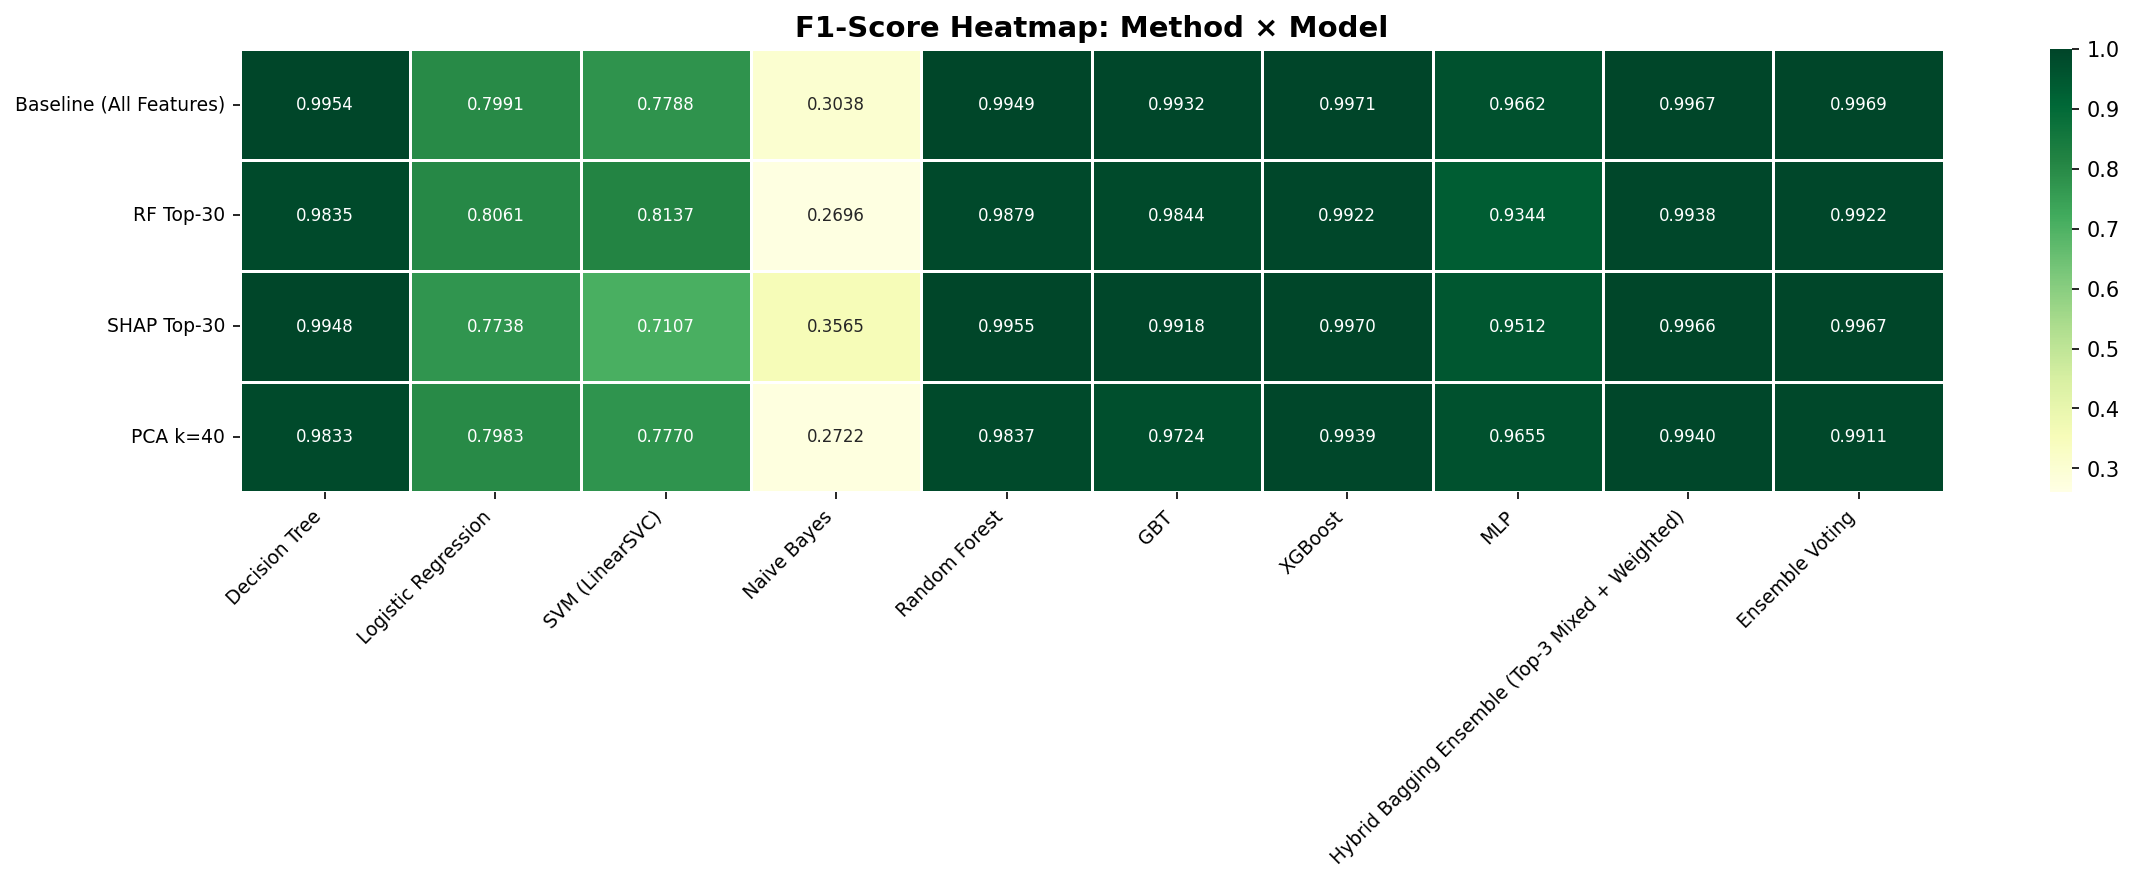
\includegraphics[width=0.95\textwidth]{f1_heatmap.png}%
  }{%
    \fbox{\parbox{0.9\textwidth}{\centering\vspace{2cm}[Hình heatmap F1]\vspace{2cm}}}%
  }
  \caption{Heatmap F1: phương pháp $\times$ thuật toán.}
  \label{fig:f1-heatmap}
\end{figure}

\begin{table}[htbp]
  \caption{Tóm tắt kết quả tốt nhất mỗi phương pháp (điền từ cross\_method\_summary.csv).}
  \label{tab:best-results}
  \centering
  \begin{tabular}{|l|l|c|c|c|}
    \hline
    Phương pháp & Mô hình & F1 & Train (s) & Size (MB) \\
    \hline
    Baseline & Decision Tree & 1.000 & 2.02 & 0.011 \\
    RF Top-30 & XGBoost & 1.000 & 6.26 & 0.257 \\
    SHAP Top-30 & XGBoost & 0.996 & 3.08 & 0.294 \\
    PCA $k$=40 & Random Forest & 0.993 & 2.71 & 0.120 \\
    \hline
  \end{tabular}
\end{table}

\subsection{Drift và robustness}

\begin{figure}[htbp]
  \centering
  \IfFileExists{../../../results/ml_07_cross_method_comparison/drift_simulation_f1.png}{%
    \includegraphics[width=0.85\textwidth]{drift_simulation_f1.png}%
  }{%
    \fbox{\parbox{0.85\textwidth}{\centering [Hình drift simulation]}}%
  }
  \caption{Mô phỏng concept drift theo các giai đoạn thời gian.}
  \label{fig:drift}
\end{figure}

\section{Thảo luận}

SHAP Top-30 cân bằng giữa F1, khả năng giải thích và số đặc trưng --- phù hợp export sang edge (30 features).
Decision Tree có kích thước mô hình nhỏ nhất, phù hợp thiết bị biên.
Triển khai phân tán trên Jetson Nano được trình bày trong công trình liên quan (SOICT 2026).

\section{Kết luận}

Bài báo so sánh bốn chiến lược giảm chiều cho IDS trên Spark ML với đánh giá drift và robustness.
Hướng phát triển: mở rộng sang RoEduNet, tối ưu hyperparameter (Exp~2), và triển khai realtime.

\begin{credits}
\subsubsection{\ackname}
Nghiên cứu được thực hiện tại Trường Đại học Giao thông Vận tải, Phân hiệu tại TP. Hồ Chí Minh
và Trường Đại học Công nghệ Thông tin, Đại học Quốc gia TP. Hồ Chí Minh,
trong khuôn khổ luận văn tốt nghiệp.

\subsubsection{\discintname}
Các tác giả không có xung đột lợi ích liên quan đến nội dung bài báo.
\end{credits}

\bibliographystyle{../../latex/splncs04}
\bibliography{references,../../latex/related_work}

\end{document}
